

% PASTA Chapter: Expanded and Enhanced
\subsection*{1. Introduction to PASTA}
The PASTA methodology (Process for Attack Simulation and Threat Analysis) represents a significant advancement in risk-centric threat modeling. Developed by Tony UcedaVélez and Marco M. Morana\cite{uceda2015}, PASTA integrates business objectives with technical analysis, enabling organizations to simulate real-world attacks and prioritize mitigations based on actual risk. Unlike traditional frameworks that focus solely on technical vulnerabilities, PASTA emphasizes the alignment of security strategies with organizational goals, regulatory requirements, and the evolving threat landscape.

\subsection*{2. Technical Definitions and Seven Stages}
PASTA is structured into seven distinct stages, each designed to provide a comprehensive view of the system and its risks:
\begin{enumerate}
	\item \textbf{Business Impact Analysis:} Identify critical assets, business goals, and compliance requirements. This ensures risk management efforts are aligned with the organization’s risk appetite and strategic objectives.
	\item \textbf{Technical Scope Definition:} Map system architecture, technologies, and interfaces. Document trust boundaries and data flows to visualize how information moves and where vulnerabilities may exist.
	\item \textbf{Application Decomposition:} Break down the application into components, subsystems, and data flows. Use Data Flow Diagrams (DFDs) and architecture diagrams to identify areas for further analysis.
	\item \textbf{Threat Analysis:} Identify potential threats using frameworks such as STRIDE, attack trees, and adversary profiles\cite{shostack2014}. Focus on how attackers might target the system and what tactics they might employ.
	\item \textbf{Vulnerability Analysis:} Assess for known and potential vulnerabilities using CVE databases, automated scanners, and code reviews\cite{owasp}. Prioritize which weaknesses need to be addressed first.
	\item \textbf{Attack Modeling:} Simulate real-world attack scenarios, leveraging penetration testing tools and adversary tactics\cite{nist800154}. Gain practical insights into how threats could materialize and their potential impact.
	\item \textbf{Risk and Impact Analysis:} Prioritize risks and develop mitigation strategies, balancing security needs with business requirements and cost considerations\cite{uceda2015}. Ensure resources are allocated effectively and significant risks are addressed.
\end{enumerate}

\begin{figure}[H]
	\centering
	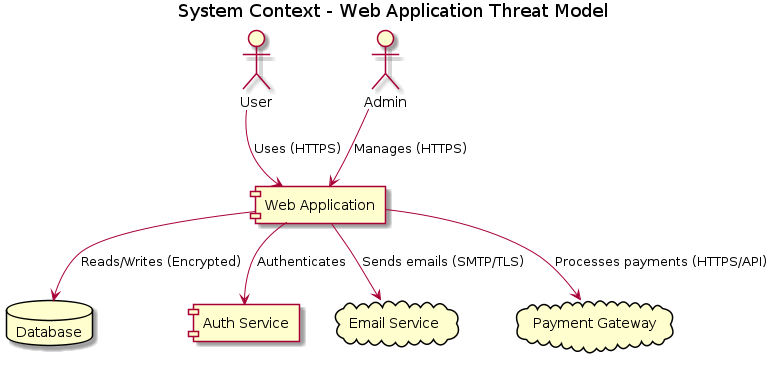
\includegraphics[width=0.8\textwidth]{images/system-context}
	\caption{PASTA Process Overview: From Business Impact to Risk Mitigation}
\end{figure}

\subsection*{3. Advantages and Practical Application}
PASTA offers several advantages over traditional threat modeling frameworks:
\begin{itemize}
	\item \textbf{Holistic Risk Management:} Integrates business and technical perspectives for a comprehensive approach.
	\item \textbf{Attacker Simulation:} Simulates realistic threats and attack paths that might otherwise be overlooked.
	\item \textbf{Risk-Based Decision Making:} Enables organizations to prioritize controls based on actual risk rather than theoretical concerns.
	\item \textbf{Scalability:} Suitable for complex, enterprise systems and environments subject to stringent regulatory requirements\cite{uceda2015}.
\end{itemize}

\subsection*{4. Implementing PASTA in the Real World}
PASTA is particularly well-suited for organizations with high-value assets, regulatory obligations, or complex threat environments. Successful implementation requires cross-functional collaboration between business, security, and technical teams. Many organizations use PASTA in conjunction with automated tools for attack simulation and vulnerability scanning, ensuring that both strategic and operational risks are addressed\cite{uceda2015,owasp}. By adopting PASTA, organizations can move beyond checkbox compliance and build security programs that are truly aligned with their business objectives.

\subsection*{5. Academic Perspective and Further Reading}
PASTA’s methodology is documented in leading books and standards. For deeper understanding, refer to:
\begin{itemize}
	\item Tony UcedaVélez and Marco M. Morana, "Risk Centric Threat Modeling" (Wiley, 2015)
	\item Adam Shostack, "Threat Modeling: Designing for Security" (Wiley, 2014)
	\item NIST SP 800-154: Guide to Data-Centric System Threat Modeling
	\item OWASP Threat Modeling Cheat Sheet
\end{itemize}
